\documentclass{article}
\usepackage{comment}
\usepackage[dvipsnames]{xcolor}
\usepackage{sectsty}
\usepackage{titlesec}
\usepackage{amssymb}
\usepackage{amsmath}
\usepackage{cancel}
\usepackage{caption}
\usepackage{subfigure}
\usepackage{tikz}
\usepackage{multicol}
\usepackage{pgfplots}
\usepackage[utf8]{inputenc}
\usepackage{amsmath}
\usepackage{amssymb}
\usepackage{graphicx}
\usepackage{float}

\setcounter{secnumdepth}{4}
\title{Computer vision - Lectures summary \\ Winter semester}

% Customize margins
\addtolength{\oddsidemargin}{-.875in}
\addtolength{\evensidemargin}{-.875in}
\addtolength{\textwidth}{1.75in}
\addtolength{\topmargin}{-.875in}
\addtolength{\textheight}{1.75in}

\titleformat{\paragraph}
{\color{blue}\normalfont\normalsize\bfseries}{\theparagraph}{1em}{}
\titlespacing*{\paragraph}
{0pt}{3.25ex plus 1ex minus .2ex}{1.5ex plus .2ex}

\sectionfont{\color{Blue}}
\subsectionfont{\color{blue}}
\subsubsectionfont{\color{blue}}

\begin{document}

\maketitle

\section{Introduction, What is camera?}

\subsection{Describe pinhole projection model}
Put a piece of film in front of an object and add a barrier to block off most of the rays.
This reduced blurring. The opening is known as the aperture. Captures pencil of rays,  all rays through a single point. This process involve a dimensional reduction (2D to 3D). We will lose the angles and
the distances but we keep the ratio of distances.

\subsection{Mention the projection properties}
\begin{itemize}
    \item \textbf{Many-to-one: } Any point along same ray maps to the same image point.
    \item \textbf{Points are mapped to points: } But only defined for points in front of
        focal plane.
    \item \textbf{Lines are mapped to lines: } Collinearity is preserved. But lines through focal
        point project to points.
    \item \textbf{Planes are mapped to planes (or half-planes): } But planes through focal point
        project to lines.
    \item \textbf{Parallel lines converge at a vanishing point: } Parallel lines converge at a
        vanishing point. But parallel lines, which are parallel to the image plane remain parallel.
        All directions in the same plane have vanishing points on the same line.
\end{itemize}

\subsection{What are some effects of vanishing projections?}
The fact of vanishing effect in projects can cause \textbf{Perspective Distortion}.

\begin{figure}[H]
\centering
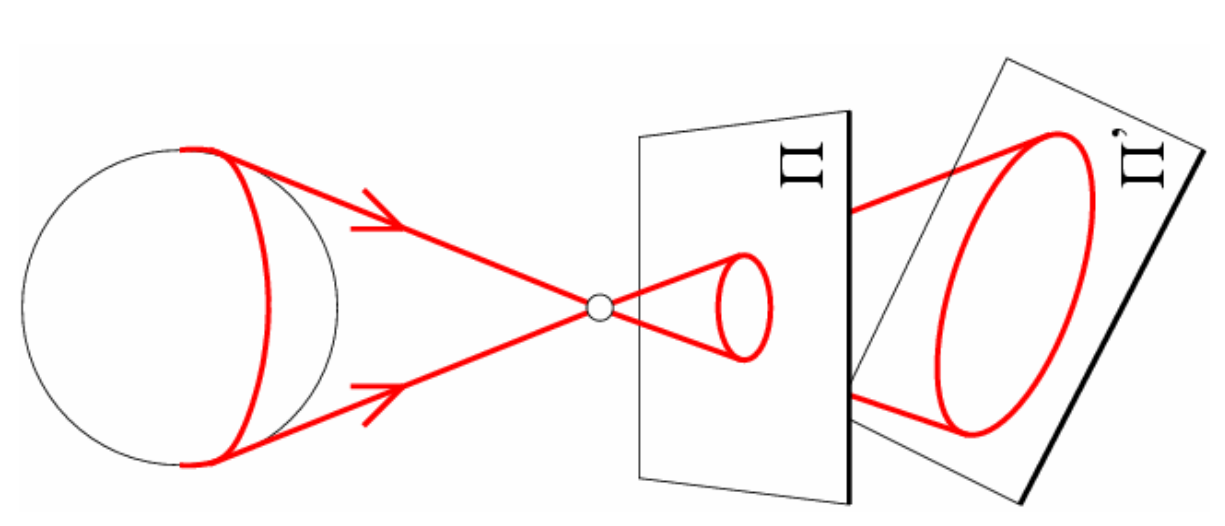
\includegraphics[scale=0.2]{pdist.png}
\caption{Perspective distortion.}
\label{fig:img2}
\end{figure}

\subsection{What is modelling projection?, and what is issue does it solve and how?}
At this point we know that the main idea of a camera is to map a 3D object to 2D image. We
know that we lose some information in this process. This mapping is possible through coordinate
projections from 3D to 2D. However we have an issue with parallel lines. We learned in school
that two parallel lines on the same plane cannot intersect never. But this is not true any more
in projective space, for example, the train railroad  becomes narrower while it moves far away
from eyes.
Taking this as context, modelling projection are some equations to know what coordinates of my object
in 3D correspond to my object in 2D.
\[P(x, y, z)^T \rightarrow (f'\frac{x}{z}, f'\frac{y}{z})^T=P'\]
Where \(P\) is my coordinate in 3D and \(P'\) in 2D. The problem is that this is \textbf{NOT A LINEAR
TRANSFORMATION}. It means that is more difficult to compute and manipulate. Homogeneous Coordinates help
us to solve this and remove the division by \(z\). This is possible adding an extra coordinate with
value 1.

\begin{figure}[H]
\centering
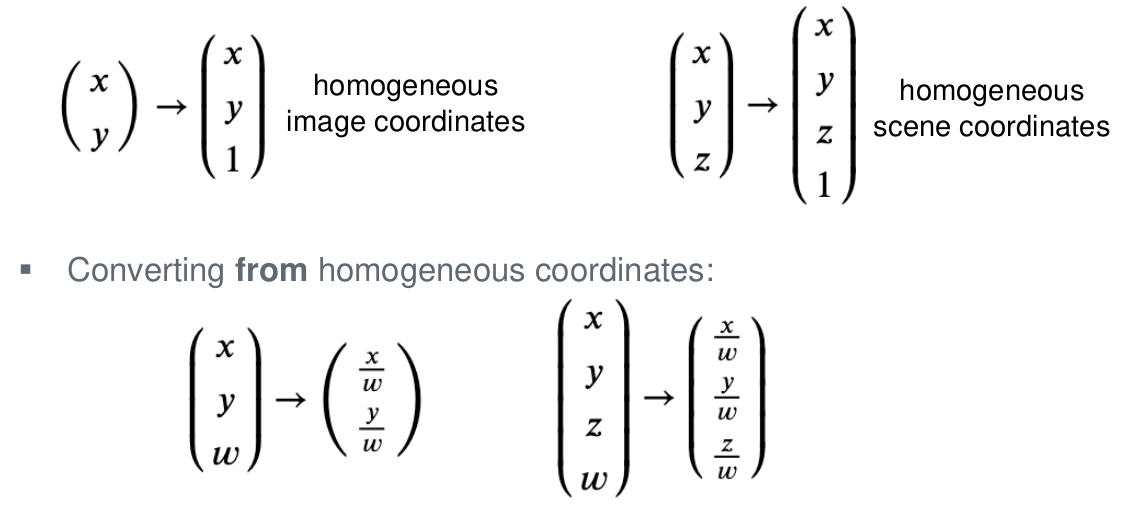
\includegraphics[scale=0.2]{homocoord.png}
\caption{Homogeneous Coordinates.}
\label{fig:img2}
\end{figure}

\subsection{What are the effects when we shrinking the Aperture?}
If our aperture is big we will get a blurred image, however if we decrease the aperture size
we can remove this blur, however if we continue decreasing the aperture to much, less light gets
through, then we will get diffraction effects.

\subsection{What do we need lens in our cameras?}
Focus all incoming light  to a point. Rays passing through the center are not deviated. All
parallel rays converge to one point (focal point) on a plane located at a distance \(f\)
\textbf{(focal length)} to the lens. There is a specific distance at which objects are in focus.
Other points project to a circle of confusion in the image.

\begin{figure}[h!]
\centering     %%% not \center
\subfigure[focus]{\label{fig:d}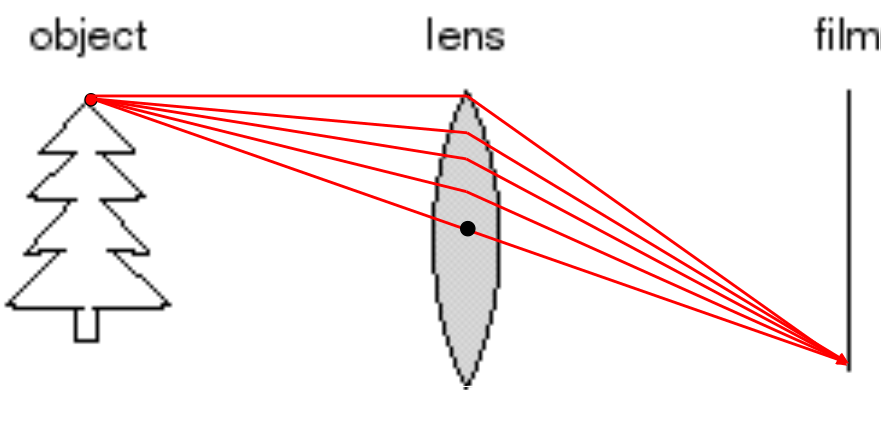
\includegraphics[width=60mm]{lens1.png}}
\subfigure[focal point]{\label{fig:e}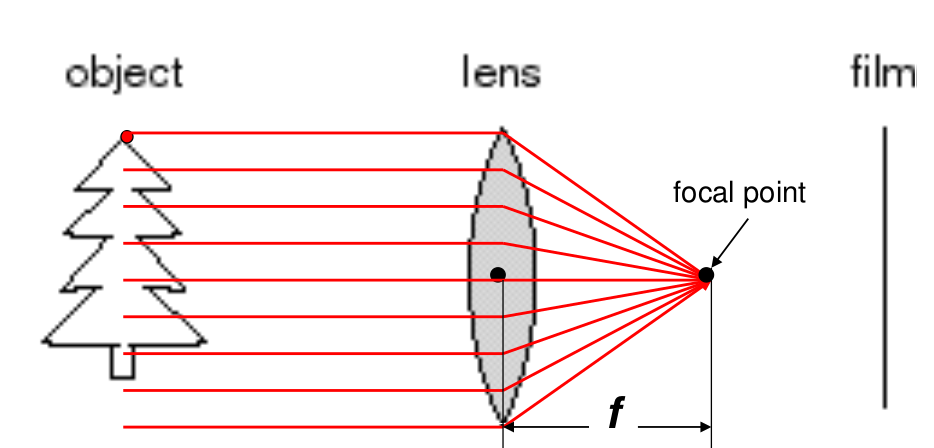
\includegraphics[width=60mm]{lens2.png}}
\subfigure[confusion]{\label{fig:f}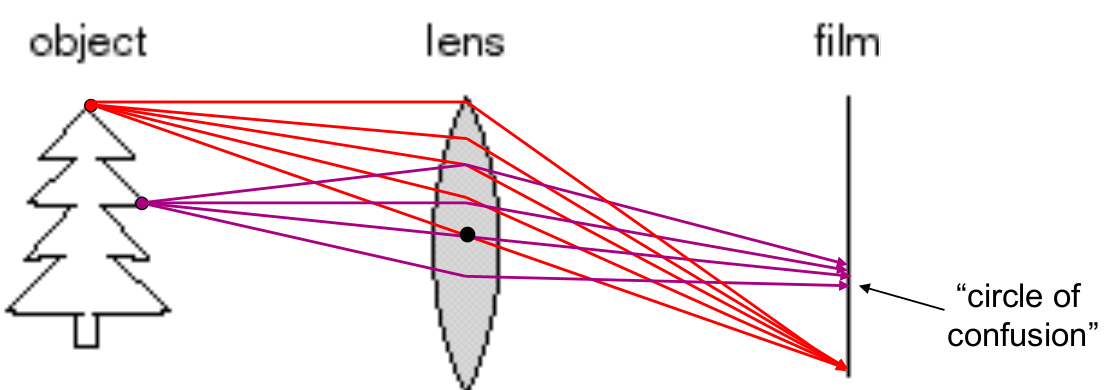
\includegraphics[width=60mm]{lens3.png}}
\caption{Lens in cameras.}
\label{fig:lens}
\end{figure}

\subsection{In order to get a sharped image, how can we calculate the distance and the focal
length?}
\[\frac{1}{D'} + \frac{1}{D} = \frac{1}{f}\]

\subsection{What is depth of field?}
Depth of field refers to the range of distance that appears acceptably sharp.

\subsection{How can we control the depth of field?}
A smaller aperture increases the range in which the object is approximately in focus. But small aperture reduces the amount of light, need to increase exposure. So, large aperture the image just focus the
nearest image and the background looks blur, smaller aperture, everything looks sharped.
\begin{itemize}
    \item Large aperture = small DOF
    \item Small aperture = large DOF
\end{itemize}

\subsection{What is Field of View?}
The area covered by an angle, \textbf{Smaller FOV = larger focal length}
\[\phi = \tan^{-1}\frac{d}{2f}\]

\begin{figure}[H]
\centering
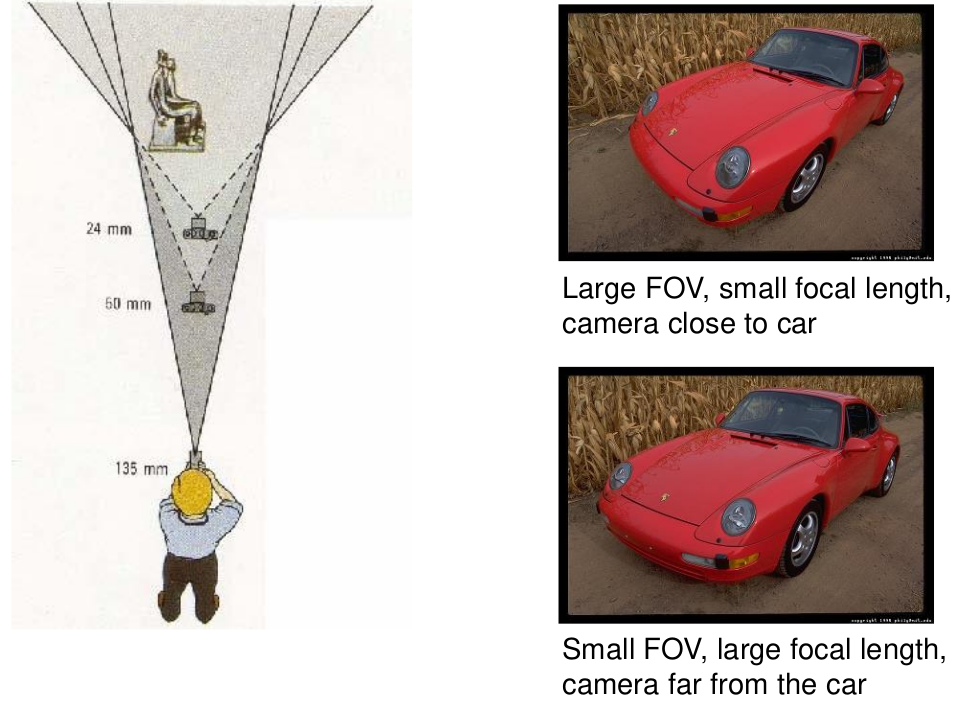
\includegraphics[scale=0.3]{FOV.png}
\caption{Field of view.}
\label{fig:img2}
\end{figure}

\subsection{Mention some lens flaws or defects}
\begin{itemize}
    \item \textbf{Chromatic Aberration:} Lens has different refractive indices for
    different wavelengths): Causes color fringing.
    \item \textbf{Lens Flaws - Vignetting:} The border of the images is dark, some light get lost
    due to the sharp of the lens.
    \item \textbf{Lens Flaws - Radial Distortion:} (Concave or convex distortion)
    Caused by imperfect lenses. Deviations are most noticeable for rays that pass through the
    edge of the lens (Pin cushion, Barrel).
\end{itemize}

\subsection{Mention the 2 technologies for digital cameras and how does it work}
A digital camera replaces film with a sensor array. Each cell in the array is a light-sensitive
diode that converts photons to electrons. There are 2 types.
\begin{itemize}
    \item \textbf{Charge coupled Devices (CCD):} transports the charge across the chip and reads
    it at one corner of the array. An analog-to-digital converter (ADC) then turns each pixel's
    value into a digital value by measuring the amount of charge at each photosite and converting
    that measurement to binary form.
    \item \textbf{Complementary metal oxide semiconductor (CMOS):} uses several transistors at
    each pixel to amplify and move the charge using more traditional wires. The CMOS signal is
    digital, so it needs no ADC.
\end{itemize}

\subsection{What is dynamic range?}
How much light a technology can capture. When the dynamic range of the scene illumination
is higher than the dynamic range of the camera, we can get under exposed areas or saturation areas.

\subsection{What are some issues with Digital Cameras}
\begin{itemize}
    \item \textbf{Noise:} Low light is where you most notice noise, Light sensitivity (ISO) / noise                tradeoff.
    \item \textbf{Resolution:} Requires higher quality lens. Noise issues
    \item \textbf{In-camera processing:} Oversharpening can produce halos.
    \item \textbf{RAW vs. compressed:} File size vs. quality tradeoff
    \item \textbf{Blooming:} Charge overflowing into neighboring pixels.
    \item \textbf{Color artifacts:} Purple fringing from microlenses, artifacts from Bayer
        patterns. White balance
\end{itemize}

\end{document}
